\subsection{Video tab}
Within the \srgui, the \textit{Vid} tab holds significant importance as it enables the viewing of camera output and adjustment of camera parameters.
This crucial functionality is depicted in Figure \ref{fig:gui_vid}.
Currently, the \srgui allows the adjustment of shutter speed and analog gain through the utilization of two sliders.
The values of these sliders are published to two topics in the \gls{pubsub} system as shown in Figure \ref{fig:pub_sub_graph}.
Adding other camera parameters to the \srgui, like color balance, is a simple task, but was not deemed necessary as they currently are kept constant during experiments.

\begin{figure}[H]
    \centering
    \begin{tabular}[b]{lr}
        \subcaptionbox{\textit{Vid} tab to see camera output adjust camera parameters.
        \label{fig:gui_vid}}{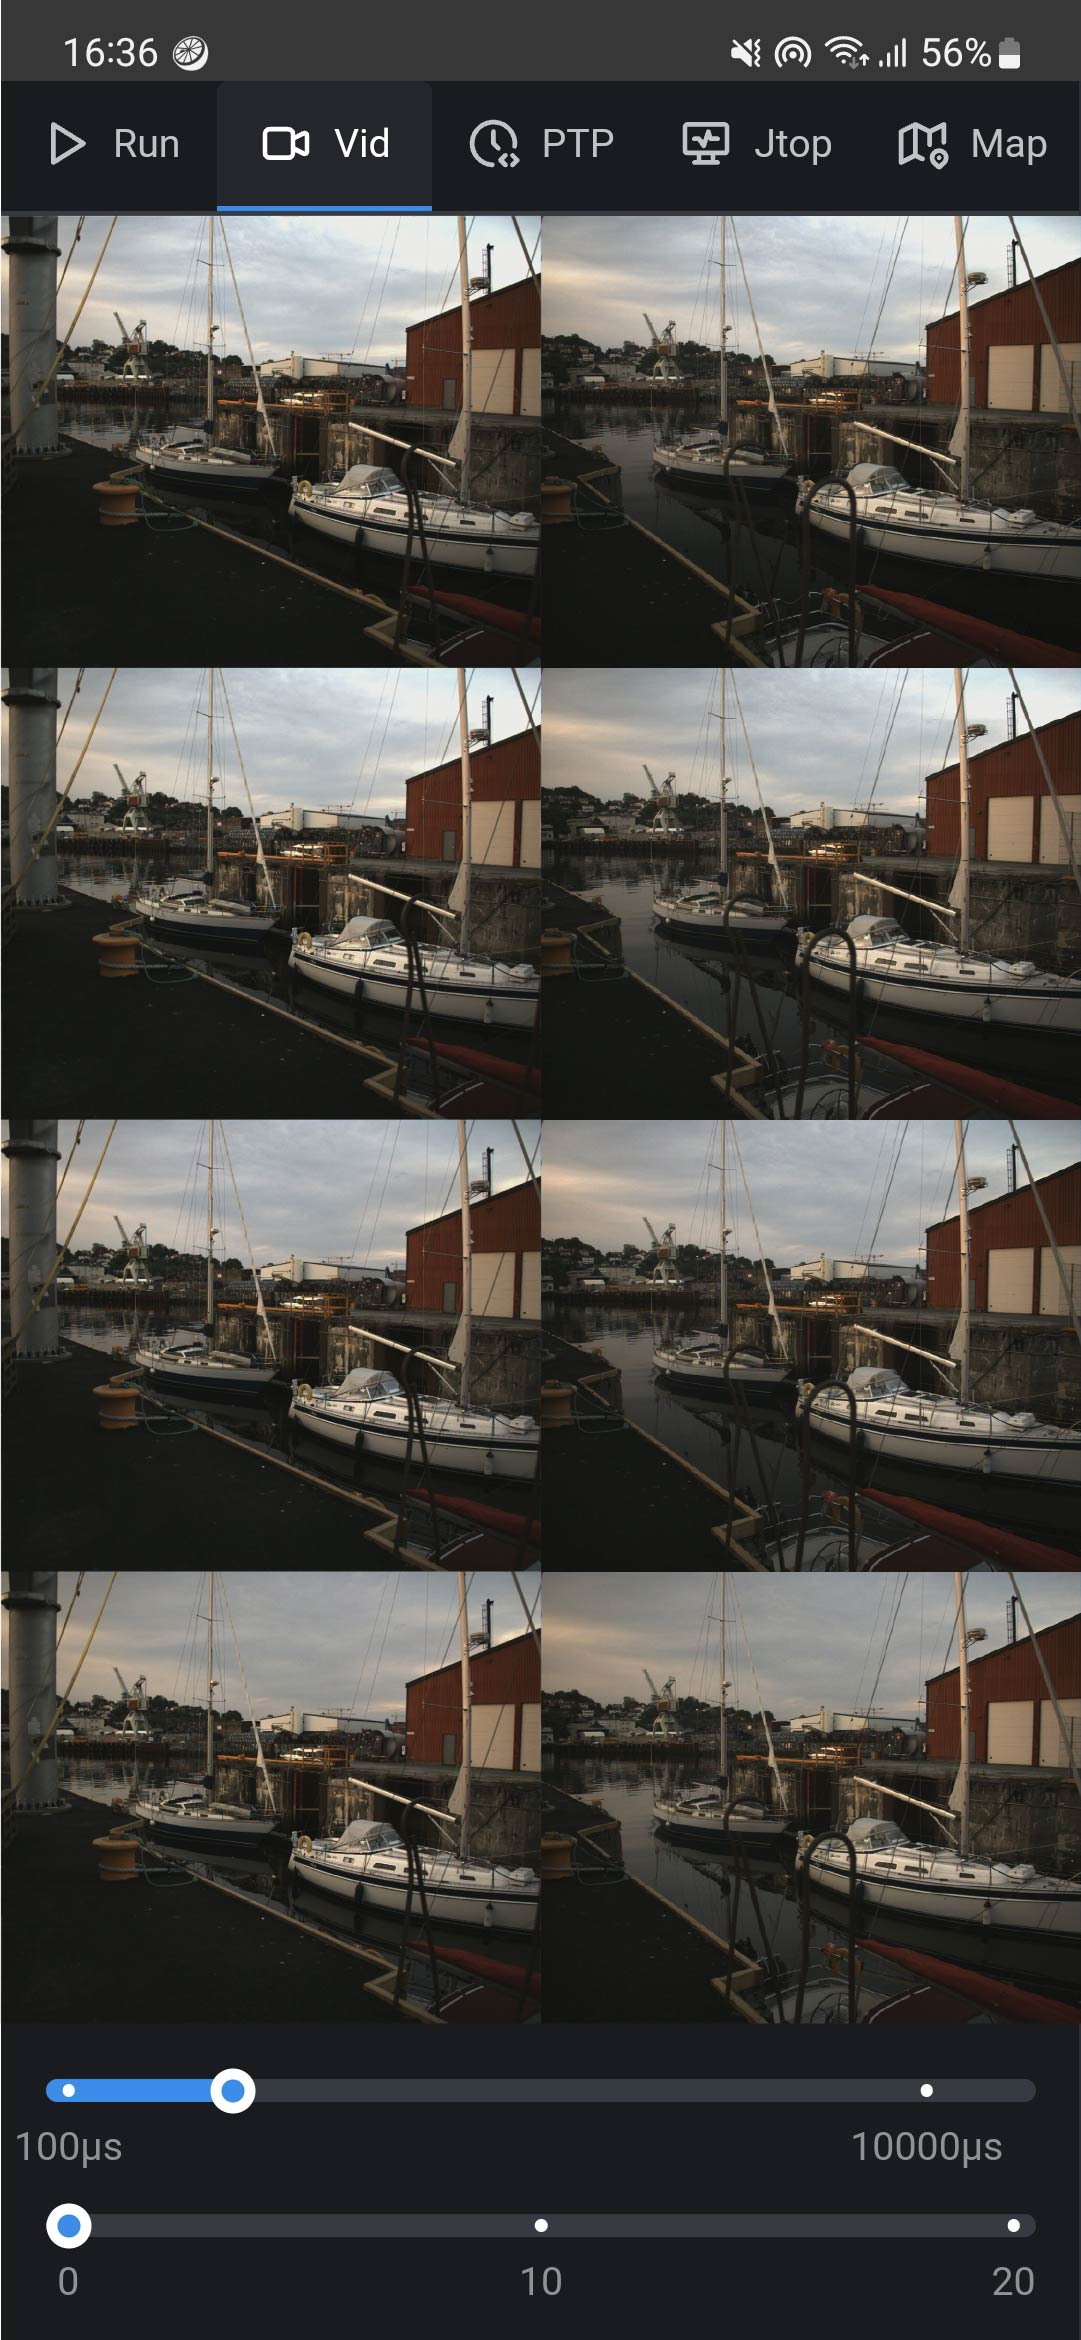
\includegraphics[width=0.48\textwidth]{figures/gui/vid.jpg}} &
        \subcaptionbox{\textit{Jtop} tab for monitoring the \jx.
            \label{fig:gui_jtop}}{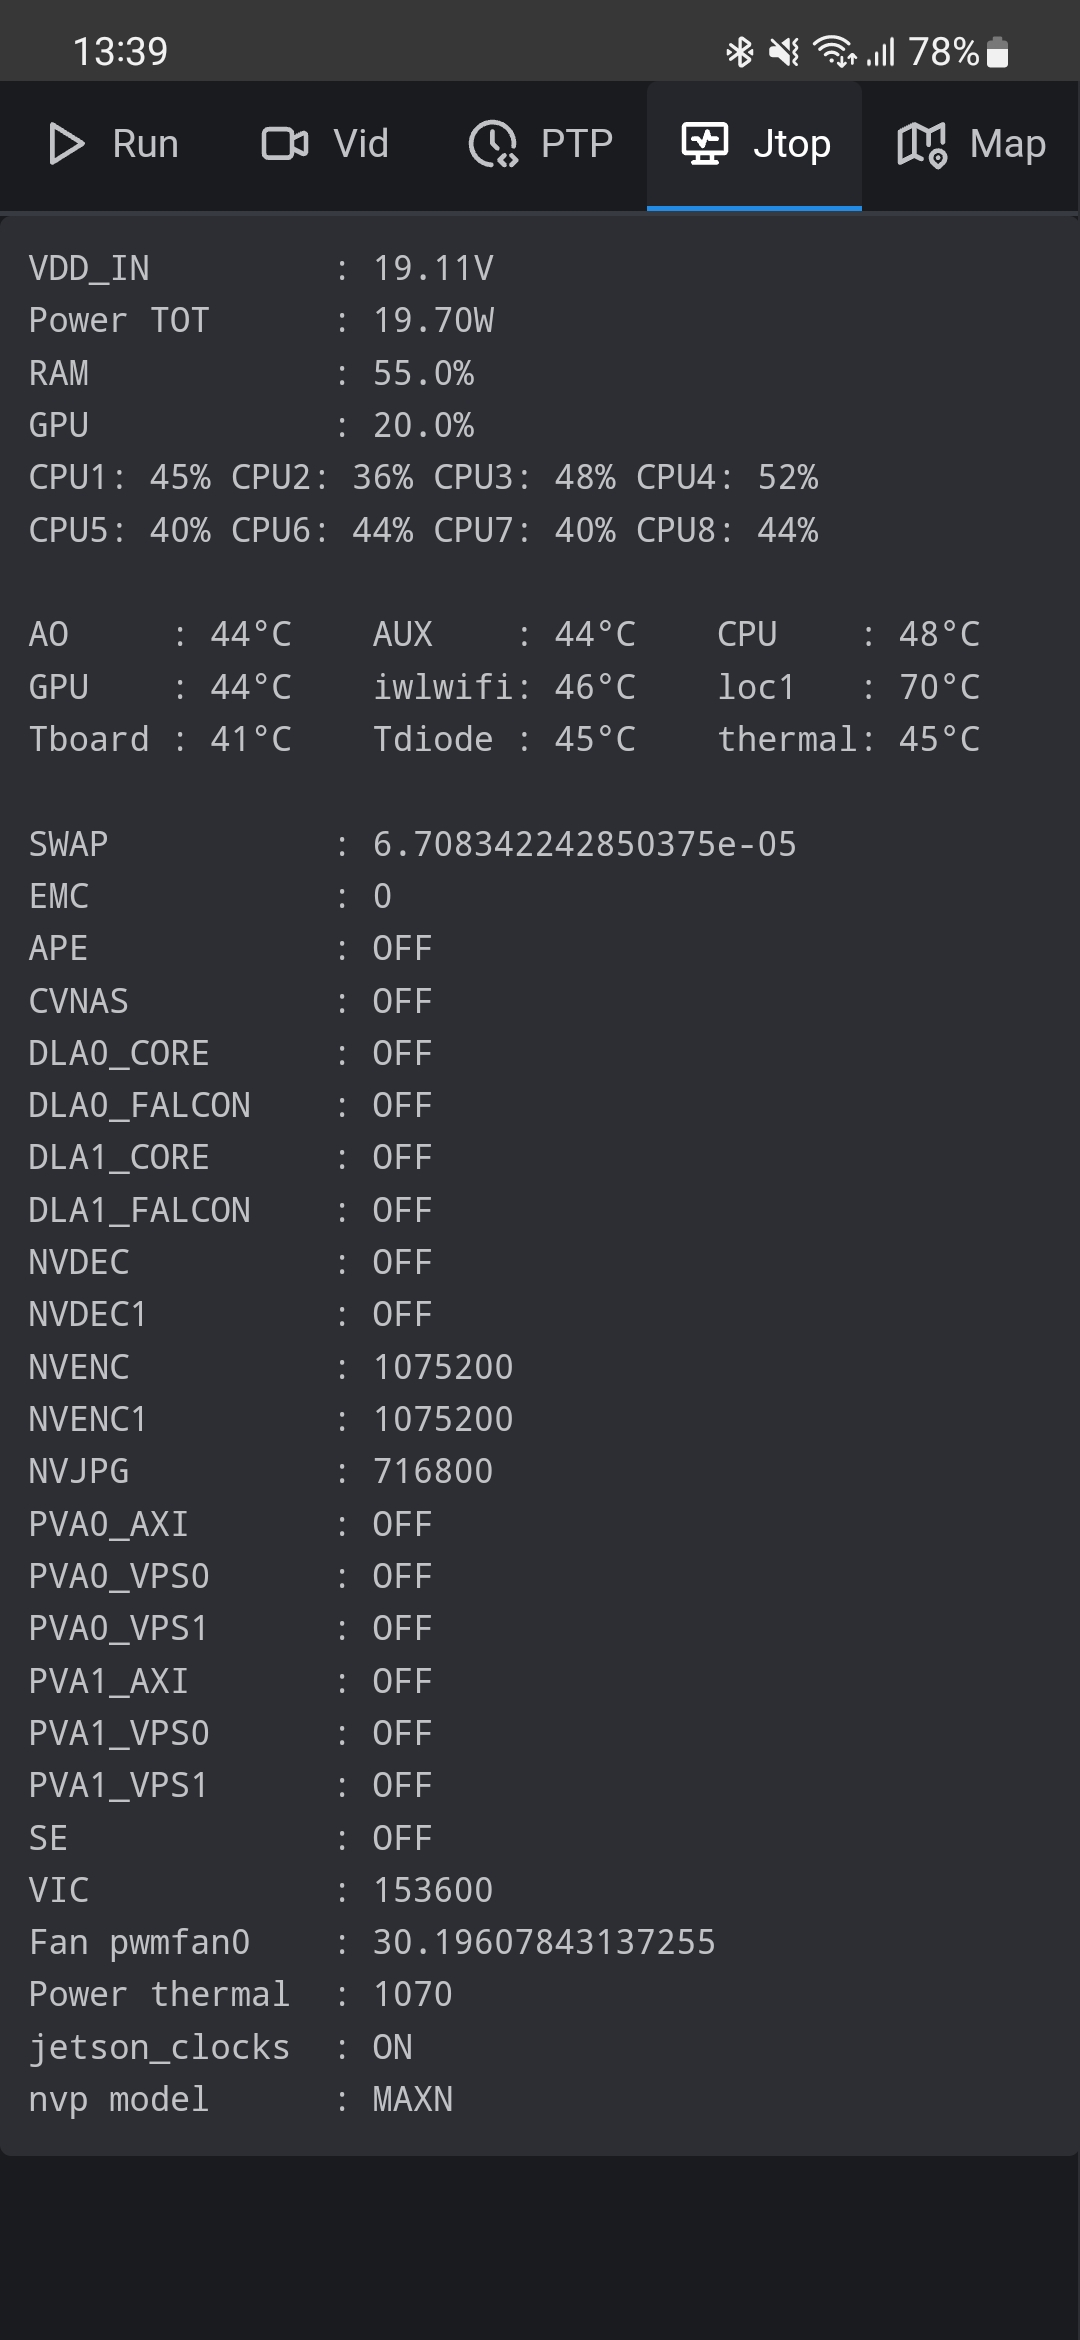
\includegraphics[width=0.48\textwidth]{figures/gui/jtop.jpg}}
    \end{tabular}
    \caption{}
\end{figure}